
\usetikzlibrary{positioning}

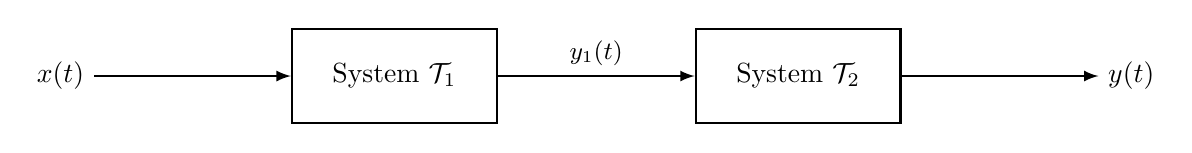
\begin{tikzpicture}[
	% Set the default distance between nodes.
	node distance=1.5cm and 2.5cm
	]
	% Define custom styles to make the code cleaner and more reusable.
	\tikzset{
		block/.style={draw, rectangle, minimum height=1.2cm, minimum width=2.6cm, align=center, thick},
		line/.style={-latex, thick} % Use -latex for a nicer arrowhead
	}
	
	% === NODES ===
	% Place the nodes for the diagram, from left to right.
	
	\node (input) {\(x(t)\)};
	\node[block, right=of input] (sys1) {System \(\mathcal{T}_1\)};
	\node[block, right=of sys1] (sys2) {System \(\mathcal{T}_2\)};
	\node[right=of sys2] (output) {\(y(t)\)};
	
	% === CONNECTIONS ===
	% Draw the lines and arrows connecting the nodes.
	
	\draw[line] (input) -- (sys1);
	\draw[line] (sys1) -- node[midway, above, font=\small] {\(y_1(t)\)} (sys2);
	\draw[line] (sys2) -- (output);
\end{tikzpicture}